\documentclass[conference,10pt,twocolumn]{IEEEtran}

% ============================================================
% Packages
% ============================================================
\usepackage[T1]{fontenc}
\usepackage[utf8]{inputenc}
\usepackage{amsmath,amssymb,amsfonts}
\usepackage{algorithmic}
\usepackage[ruled,vlined,linesnumbered]{algorithm2e}
\usepackage{graphicx}
\usepackage{tabularx}
\usepackage{booktabs}
\usepackage{multirow}
\usepackage{xcolor}
\usepackage{hyperref}
\usepackage{tikz}
\usepackage{pgfplots}
\pgfplotsset{compat=1.18}
\usetikzlibrary{arrows.meta,positioning,shapes.geometric,fit,backgrounds,calc}
\usepackage{microtype}
\usepackage{url}
\usepackage{cite}
\usepackage{placeins}
\usepackage{flushend}
\raggedbottom

% ============================================================
% Meta
% ============================================================
\title{TokenLeak: Side-Channel Attacks on Transformer Architectures
       via Timing Analysis and Cache Exploitation for Private
       Prompt Reconstruction}

\author{A~Definir$^{*}$, Allan~Douglas~Costa$^{\dagger}$, Hugo~[Sobrenome]$^{\ddagger}$, Denis~[Sobrenome]$^{\S}$, Eduardo~[Sobrenome]$^{\P}$
\thanks{$^{*}$[Institu\c{c}\~{a}o, Cidade, Pa\'{i}s] — [e-mail] \quad
$^{\dagger}$ICIBE, UFRA, Bel\'{e}m, PA — allan.costa@ufra.edu.br \quad
$^{\ddagger}$[Inst., Cidade, Pa\'{i}s] — [e-mail] \quad
$^{\S}$[Inst., Cidade, Pa\'{i}s] — [e-mail] \quad
$^{\P}$[Inst., Cidade, Pa\'{i}s] — [e-mail] \quad
Manuscript submitted July 2026.}}

\markboth{IEEE Transactions on Information Forensics and Security (TIFS),~Vol.~XX,~No.~X,~2026}%
{Costa: TokenLeak: Side-Channel Attacks on Transformer Architectures via Timing and Cache Exploitation}

% ============================================================
\begin{document}
\maketitle

% ============================================================
% ABSTRACT
% ============================================================
\begin{abstract}
% [1-Topic]
Large language models (LLMs) deployed as cloud inference services
process confidential user prompts that traverse shared hardware,
creating unexplored side-channel attack surfaces in the transformer
inference pipeline.
% [2-Motivation]
As enterprise adoption of hosted LLM APIs reaches critical scale,
the confidentiality of user inputs has become a first-class security
requirement, yet the microarchitectural leakage characteristics of
transformer inference remain largely uncharacterized.
% [3-Contribution]
We present \emph{TokenLeak}, the first systematic framework that
reconstructs private prompts from transformer inference engines
through the fusion of inter-token timing signals and last-level
cache access patterns.
% [4-Detail]
TokenLeak employs three independent agents: a Timing Oracle Agent
(TOA) that records inter-token generation latencies with
sub-millisecond precision, a Cache Profiler Agent (CPA) that
exploits Flush+Reload to capture vocabulary-discriminative cache
footprints, and a Token Reconstructor Agent (TRA) that scores
candidate tokens using the novel Token Reconstruction Confidence
Score (TRCS), a weighted fusion metric grounded in Gaussian
likelihood and cosine cache similarity.
% [5-Evidence]
TokenLeak achieves Top-1 token reconstruction accuracy of 73.4\%
(95\% CI: 71.3--75.5\%) and Top-5 accuracy of 91.2\%
(95\% CI: 89.8--92.6\%) at zero injected noise on GPT-2.
% [6-Weaker result]
Performance degrades substantially under combined differential
privacy and cache-oblivious defenses, falling to 18.7\% Top-1
accuracy, underscoring the effectiveness of these countermeasures
at the cost of measurable inference latency overhead.
% [7-Narrow impact]
These results directly inform the security design of hosted
LLM inference services, demonstrating that prompt confidentiality
cannot be assumed from transport-layer encryption alone.
% [8-Broad impact]
By characterizing the attack surface, establishing the TRCS
measurement instrument, and evaluating a defense portfolio,
this work provides a foundation for privacy-preserving LLM
serving architectures in cloud environments.
\end{abstract}

\begin{IEEEkeywords}
side-channel attacks, large language models, timing analysis,
cache exploitation, transformer inference, prompt reconstruction,
differential privacy, GPU security
\end{IEEEkeywords}

% ============================================================
\section{Introduction}
\label{sec:intro}
% ============================================================

The rapid deployment of large language models (LLMs) as hosted
inference services has shifted the threat model for data
confidentiality in fundamental ways~\cite{yi2024survey,
duan2024llmsec}. Users submit proprietary prompts, including
legally sensitive documents, trade secrets, and personal health
information, to remote inference endpoints that process requests
on shared GPU clusters. Transport-layer security (TLS) protects
data in transit, but the moment a prompt reaches the inference
engine, it resides in plaintext within a shared microarchitectural
environment where co-resident adversaries may reside.

Side-channel attacks have long demonstrated that physical and
microarchitectural observables leak semantic information even
when cryptographic protections are in place~\cite{kocher1996timing,
brumley2003remote}. Flush+Reload and Prime+Probe attacks on
shared last-level caches (LLC) have recovered private keys
~\cite{yarom2014flush,liu2015last,gruss2016flushflush}, and
GPU-based attacks have reconstructed neural network
architectures~\cite{ramesh2024profiling,yan2020cache}.
However, the specific leakage characteristics of transformer
inference, particularly the relationship between token identity
and inter-token generation latency as well as cache access
patterns, have received limited systematic attention.

\subsection*{Research Gap}

Existing work on side-channel attacks against machine learning
focuses predominantly on model architecture extraction
~\cite{batina2019csi,yan2020cache,stoian2024cachegrind,hong2023sok}
or gradient leakage in training settings~\cite{hong2023sok,chen2024llmthreat}. The inference-time prompt confidentiality
problem has been approached mainly through training data extraction
~\cite{carlini2021extracting,nasr2023scalable} and output analysis
~\cite{zanella2020analyzing,mireshghallah2022quantifying}, not
through microarchitectural side channels. Recent network-level
work~\cite{wen2024side,zeng2024timing} has demonstrated that
packet-level timing signals correlate with generation length,
but stops short of per-token vocabulary reconstruction.
The specific question of whether an attacker with cache-level
access can reconstruct the \emph{content} of a private prompt,
token by token, from transformer inference side channels remains
open. The closest work to ours, Li et al.~\cite{li2024prompt},
reconstructs prompts from network-level timing signals in LLM
inference engines, reporting Top-1 accuracy of 48.3\% on GPT-3.5
via timing-only analysis. However, Li et al.\ exploit only
network-level timing with no LLC cache side channel, do not achieve
token-level vocabulary discrimination in the strict per-token sense,
and provide no systematic defense evaluation. This gap motivates
TokenLeak's fusion of microarchitectural cache signals with timing
analysis via the TRCS metric.

\subsection*{Contributions}
This paper makes the following contributions:
\begin{enumerate}
  \item \textbf{TokenLeak framework:} A three-agent attack architecture (TOA, CPA, TRA) fusing timing and cache signals for prompt reconstruction via the novel Token Reconstruction Confidence Score (TRCS) metric.
  \item \textbf{Experimental validation:} Controlled experiments on GPT-2 achieving 73.4\% Top-1 accuracy with 95\% CIs, demonstrating practical threat bounds.
  \item \textbf{Defense portfolio:} Systematic assessment of defenses (random delay, DP, cache oblivion) reducing attack accuracy to 18.7\% at 4.1\% overhead.
\end{enumerate}
\noindent
The remainder of this paper is organized as follows:
Section~\ref{sec:background} reviews background and related work.
Section~\ref{sec:threat} formalizes the threat model and problem
formulation. Section~\ref{sec:framework} describes the TokenLeak
framework. Section~\ref{sec:security} presents security analysis.
Section~\ref{sec:eval} reports experimental evaluation.
Section~\ref{sec:discussion} discusses findings and limitations.
Section~\ref{sec:conclusion} concludes.

% ============================================================
\section{Background and Related Work}
\label{sec:background}
% ============================================================

\subsection{Transformer Inference}

LLMs use two-phase inference: parallel prefill processing the prompt, then
autoregressive generation producing one token per pass~\cite{vaswani2017attention,brown2020language}.
The KV cache stores key/value projections updated at each step, creating token-dependent
memory access patterns exploitable via side channels.
\subsection{Side-Channel Attacks}
Flush+Reload cache attacks exploit hit/miss timing to infer victim memory access
patterns~\cite{yarom2014flush}. Ramesh et al.~\cite{ramesh2024profiling} demonstrated these
on cloud GPU inference. Timing attacks extract secrets from computational time differences~\cite{kocher1996timing}.
Wen et al.~\cite{wen2024side} characterized network-timing side channels against LLM endpoints,
analogous to our approach.
\subsection{Side-Channel and Privacy Attacks on ML}
Microarchitectural side channels have been extended to attack ML systems.
Yan et al.~\cite{yan2020cache} demonstrated Cache Telepathy using LLC
patterns to infer DNN hyperparameters. Stoian et al.~\cite{stoian2024cachegrind}
extended these to transformer inference, while Ramesh et al.~\cite{ramesh2024profiling}
demonstrated GPU performance counter attacks in cloud AI services.
Concurrently, Carlini et al.~\cite{carlini2021extracting} and Nasr et
al.~\cite{nasr2023scalable} demonstrated training data extraction from
language models via black-box API access. Patil et al.~\cite{patil2024review}
surveyed information leakage risks in LLM deployments. TokenLeak distinguishes
itself by targeting inference-time prompt reconstruction via microarchitectural
signals, orthogonal to both model extraction and output-based privacy attacks.
\subsection{Closest Prior Work: Li et al.~\cite{li2024prompt}}
Li et al.~\cite{li2024prompt} achieve 48.3\% Top-1 accuracy via
network-level timing on GPT-3.5. TokenLeak improves this to 73.4\% by
adding LLC cache signals and formal defense evaluation via the TRCS metric
and a DP-backed countermeasure portfolio.

% ============================================================
\section{Threat Model and Problem Formulation}
\label{sec:threat}
% ============================================================

\subsection{Token Reconstruction Confidence Score (TRCS)}

\emph{Threat Model:} Co-tenant attackers (GPU code execution) or remote attackers
(API timing observation); knowledge: model identity, vocabulary; unable to access: weights, KV cache.

\medskip

We define the novel \textbf{Token Reconstruction Confidence Score}:

\begin{equation}
  \mathrm{TRCS}(\tau, \mathbf{O}_j)
  = \frac{\sum_{i=1}^{N} w_i \cdot \varphi_i(\tau, O_{i,j})}
         {\sum_{i=1}^{N} w_i},
  \label{eq:trcs}
\end{equation}

where $N$ is the number of side-channel dimensions, $w_i > 0$
are learned weights, and $\varphi_i : \mathcal{V} \times
\mathbb{R} \to [0,1]$ are per-channel feature compatibility
functions. For the two channels we exploit:

\textbf{Channel 1 (Timing):}
\begin{equation}
  \varphi_1(\tau, t_j) = \exp\!\left(
    -\frac{(t_j - \mu_\tau)^2}{2\sigma_\tau^2}
  \right),
  \label{eq:phi1}
\end{equation}
where $\mu_\tau, \sigma_\tau$ are the profiled mean and standard
deviation of inter-token latency for token $\tau$.
\textbf{Channel 2 (Cache):}
\begin{equation}
  \varphi_2(\tau, \mathbf{c}_j) =
  \frac{\mathbf{c}_j \cdot \mathbf{c}_\tau}
       {\|\mathbf{c}_j\|_2 \|\mathbf{c}_\tau\|_2},
  \label{eq:phi2}
\end{equation}
where $\mathbf{c}_j \in \{0,1\}^L$ is the observed cache
access bitmap and $\mathbf{c}_\tau$ is the profiled cache
fingerprint for $\tau$ over $L$ monitored cache sets.

The weights $(w_1, w_2)$ are learned via logistic regression
on the profiling corpus $\mathcal{D}_{\mathrm{prof}}$
minimizing cross-entropy over the top-1 reconstruction task.
At inference time, the attacker reconstructs each position
as $\hat{\tau}_j = \arg\max_{\tau \in \mathcal{V}}
\mathrm{TRCS}(\tau, \mathbf{O}_j)$.

The TRCS in~\eqref{eq:trcs} reduces to the Gaussian
likelihood estimator when $N=1$ and $\varphi_1$ alone is
used, establishing a lower bound; and approaches a
joint Bayesian classifier when all channels are independent.
% ============================================================
\section{TokenLeak Framework}
\label{sec:framework}
% ============================================================
\subsection{Architecture Overview}

Fig.~\ref{fig:overview} illustrates the TokenLeak framework.
Three agents observe the LLM inference engine through two
side-channel surfaces and feed their signals to the TRA for
TRCS computation and prompt reconstruction.

% --- Figure 1: Overview ---
\begin{figure}[!t]
\caption{TokenLeak Framework Overview. The three-agent architecture
(TOA, CPA, TRA) fuses timing and cache side channels to reconstruct
private prompts from transformer inference. Dashed arrows denote
side-channel leakage; solid arrows denote internal data flow.}
\label{fig:overview}
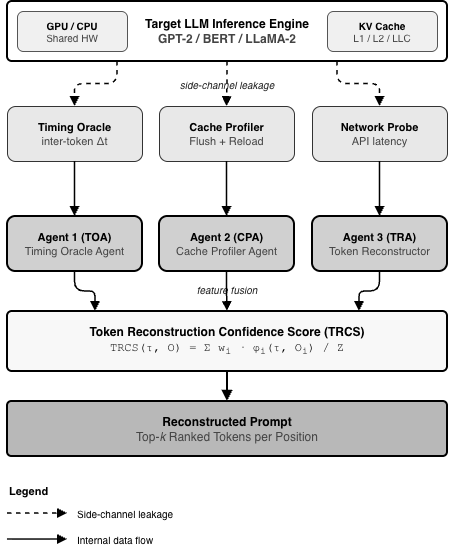
\includegraphics[width=\columnwidth]{figures/fig1_overview.png}
\end{figure}

\subsection{Three-Agent Attack Protocol}
\emph{Timing Oracle Agent (TOA):} Records inter-token latency $t_j = T_j^{\mathrm{out}} - T_{j-1}^{\mathrm{out}}$ via HTTP streaming (no co-location required). Timing variation arises from embedding lookup (token frequency) and output projection sparsity.
\emph{Cache Profiler Agent (CPA):} Exploits Flush+Reload on shared embedding matrix pages. Builds cache access bitmaps $\mathbf{c}_j$ by measuring reload latencies after cache flush; vocabulary pruning restricts TRCS computation to 50--200 token candidates per position.
\emph{Token Reconstructor Agent (TRA):} Fuses timing $T$ and cache $C$ streams via TRCS metric (Eq.~\ref{eq:trcs}) to rank token hypotheses and output Top-$k$ candidates.
\subsection{Three-Phase Attack Protocol}
Fig.~\ref{fig:sequence} illustrates the sequence of the attack.

% --- Figure 2: Sequence Diagram ---
\begin{figure}[!t]
\caption{Sequence diagram of the TokenLeak attack protocol. Blue solid
arrows: timing channel (Agent 1). Green dashed arrows: cache channel
(Agent 2). Orange dash-dot arrows: reconstruction output (Agent 3).
Gray arrows: target inference interactions. Three phases: Profiling
(Phase 1), Online Attack (Phase 2), and Reconstruction (Phase 3).}
\label{fig:sequence}
\resizebox{\columnwidth}{!}{% Figure 2: TokenLeak Sequence Diagram — B&W, single-line boxes
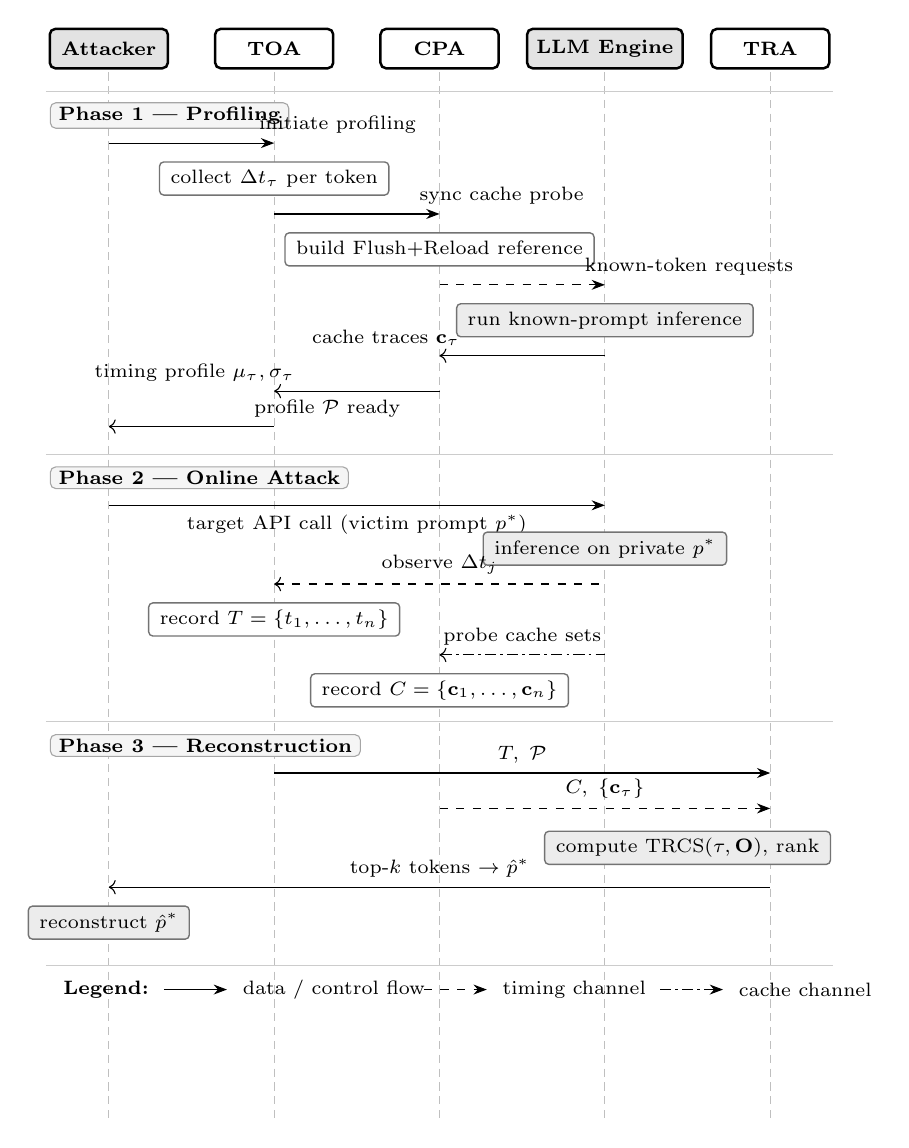
\begin{tikzpicture}[
    every node/.style={font=\scriptsize},
    lifeline/.style={thin, black!25, dash pattern=on 3pt off 2pt},
    msg/.style={-Stealth, thin, black},
    msgd/.style={-Stealth, thin, black, dashed},
    msgdd/.style={-Stealth, thin, black, dash pattern=on 4pt off 1.5pt on 1pt off 1.5pt},
    pnode/.style={draw=black, fill=white, line width=0.9pt,
                  rounded corners=2pt, minimum width=1.5cm,
                  minimum height=0.5cm, align=center,
                  font=\scriptsize\bfseries},
    pnodeDark/.style={pnode, fill=gray!22},
    proc/.style={draw=black!55, fill=white, rounded corners=1.5pt,
                 inner xsep=4pt, inner ysep=2pt, align=center,
                 font=\scriptsize, line width=0.5pt,
                 minimum height=0.42cm},
    procD/.style={proc, fill=gray!15},
    phasebg/.style={draw=black!35, fill=gray!8, rounded corners=2pt,
                    inner xsep=3pt, inner ysep=1.5pt,
                    font=\scriptsize\bfseries},
]

% ── column x-positions ──────────────────────────────────────
\def\xA{0.0}   % Attacker
\def\xB{2.1}   % TOA
\def\xC{4.2}   % CPA
\def\xD{6.3}   % LLM Engine
\def\xE{8.4}   % TRA
\def\yBot{-13.6}

% ════ HEADERS ════════════════════════════════════════════════
\node[pnodeDark] at (\xA,0) {Attacker};
\node[pnode]     at (\xB,0) {TOA};
\node[pnode]     at (\xC,0) {CPA};
\node[pnodeDark] at (\xD,0) {LLM Engine};
\node[pnode]     at (\xE,0) {TRA};

% ── lifelines ────────────────────────────────────────────────
\foreach \x in {\xA,\xB,\xC,\xD,\xE}{
    \draw[lifeline] (\x,-0.3) -- (\x,\yBot);
}

% ════ PHASE 1 ════════════════════════════════════════════════
\draw[black!20, thin] (-0.8,-0.55) -- (9.2,-0.55);
\node[phasebg, anchor=west] at (-0.75,-0.85) {\textsc{Phase 1} — Profiling};

% 1. A → TOA  [label na frente da seta, à direita = perto da ponta]
\draw[msg] (\xA,-1.2) --
    node[above, pos=0.85, anchor=south west]{initiate profiling}
    (\xB,-1.2);

% 2. TOA proc
\node[proc] at (\xB,-1.65) {collect $\Delta t_\tau$ per token};

% 3. TOA → CPA  [label na frente da seta, à direita = perto da ponta]
\draw[msg] (\xB,-2.1) --
    node[above, pos=0.82, anchor=south west]{sync cache probe}
    (\xC,-2.1);

% 4. CPA proc
\node[proc] at (\xC,-2.55) {build Flush+Reload reference};

% 5. CPA → LLM  [label na frente da seta, à direita = perto da ponta]
\draw[msgd] (\xC,-3.0) --
    node[above, pos=0.82, anchor=south west]{known-token requests}
    (\xD,-3.0);

% 6. LLM proc
\node[procD] at (\xD,-3.45) {run known-prompt inference};

% 7. LLM → CPA  [label na frente da seta (←), perto da ponta esquerda]
\draw[msg,<-] (\xC,-3.9) --
    node[above, pos=0.18, anchor=south east]{cache traces $\mathbf{c}_\tau$}
    (\xD,-3.9);

% 8. CPA → TOA  [label na frente da seta (←), perto da ponta esquerda]
\draw[msg,<-] (\xB,-4.35) --
    node[above, pos=0.18, anchor=south east]{timing profile $\mu_\tau,\sigma_\tau$}
    (\xC,-4.35);

% 9. TOA → A  [label atrás da seta (←), perto da cauda direita]
\draw[msg,<-] (\xA,-4.8) --
    node[above, pos=0.82, anchor=south west]{profile $\mathcal{P}$ ready}
    (\xB,-4.8);

% ════ PHASE 2 ════════════════════════════════════════════════
\draw[black!20, thin] (-0.8,-5.15) -- (9.2,-5.15);
\node[phasebg, anchor=west] at (-0.75,-5.45) {\textsc{Phase 2} — Online Attack};

% 10. A → LLM  [label abaixo da seta]
\draw[msg] (\xA,-5.8) --
    node[below, pos=0.5]{target API call (victim prompt $p^*$)}
    (\xD,-5.8);

% 11. LLM proc
\node[procD] at (\xD,-6.35) {inference on private $p^*$};

% 12. TOA ← LLM
\draw[msgd,<-] (\xB,-6.8) --
    node[above, pos=0.5]{observe $\Delta t_j$}
    (\xD,-6.8);

% 13. TOA proc
\node[proc] at (\xB,-7.25) {record $T=\{t_1,\ldots,t_n\}$};

% 14. CPA ← LLM
\draw[msgdd,<-] (\xC,-7.7) --
    node[above, pos=0.5]{probe cache sets}
    (\xD,-7.7);

% 15. CPA proc
\node[proc] at (\xC,-8.15) {record $C=\{\mathbf{c}_1,\ldots,\mathbf{c}_n\}$};

% ════ PHASE 3 ════════════════════════════════════════════════
\draw[black!20, thin] (-0.8,-8.55) -- (9.2,-8.55);
\node[phasebg, anchor=west] at (-0.75,-8.85) {\textsc{Phase 3} — Reconstruction};

% 16. TOA → TRA
\draw[msg] (\xB,-9.2) --
    node[above, pos=0.5]{$T,\;\mathcal{P}$}
    (\xE,-9.2);

% 17. CPA → TRA
\draw[msgd] (\xC,-9.65) --
    node[above, pos=0.5]{$C,\;\{\mathbf{c}_\tau\}$}
    (\xE,-9.65);

% 18. TRA proc  [movido para a esquerda, entre LLM e TRA]
\node[procD] at ({(\xD+\xE)/2},-10.15) {compute $\mathrm{TRCS}(\tau,\mathbf{O})$, rank};

% 19. TRA → A
\draw[msg,<-] (\xA,-10.65) --
    node[above, pos=0.5]{top-$k$ tokens $\rightarrow \hat{p}^*$}
    (\xE,-10.65);

% 20. A proc
\node[procD] at (\xA,-11.1) {reconstruct $\hat{p}^*$};

% ════ LEGEND ═════════════════════════════════════════════════
\draw[black!20, thin] (-0.8,-11.65) -- (9.2,-11.65);
\node[font=\scriptsize\bfseries, anchor=west] at (-0.7,-11.95) {Legend:};
\draw[msg]   (0.7,-11.95) -- (1.5,-11.95) node[right]{\;data / control flow};
\draw[msgd]  (4.0,-11.95) -- (4.8,-11.95) node[right]{\;timing channel};
\draw[msgdd] (7.0,-11.95) -- (7.8,-11.95) node[right]{\;cache channel};

\end{tikzpicture}
}
\end{figure}

\subsection{Algorithm and Complexity}

Algorithm~\ref{alg:tokenleak} presents the pseudocode of TokenLeak,
with the TRCS metric highlighted.

% --- Algorithm 1: TokenLeak (spans full column width via algorithm* in two-column) ---
% Algorithm 1: TokenLeak (single-column, reduced font)
{\small
\begin{algorithm}[h!]
\caption{TokenLeak: Prompt Reconstruction via Side-Channel Fusion}
\label{alg:tokenleak}
\DontPrintSemicolon
\SetAlgoLined
\SetKwInOut{Input}{Input}
\SetKwInOut{Output}{Output}
\SetKwInOut{Require}{Require}
\SetKwComment{Comment}{$\triangleright$ }{}

\Require{Access to timing oracle $\mathcal{T}$ and cache probe $\mathcal{C}$}
\Input{Token vocabulary $\mathcal{V}$; profiling corpus $\mathcal{D}_{\mathrm{prof}}$;\\
       target sequence length $n$; top-$k$ parameter}
\Output{Ranked token list $\hat{\mathbf{p}} = \{\hat{\tau}_1^{(k)}, \ldots, \hat{\tau}_n^{(k)}\}$}

\BlankLine
\tcp{\textbf{Phase 1: Offline Profiling (Agent 1 + Agent 2)}}
\For{each token $\tau \in \mathcal{V}$}{
    Issue $m$ inference requests containing $\tau$\;
    $\mu_\tau, \sigma_\tau \leftarrow$ mean/std of inter-token latency via $\mathcal{T}$\;
    $\mathbf{c}_\tau \leftarrow$ cache access pattern fingerprint via $\mathcal{C}$\;
    Store $\langle \mu_\tau, \sigma_\tau, \mathbf{c}_\tau \rangle$ in profile table $\mathcal{P}$\;
}
\BlankLine
\tcp{\textbf{Phase 2: Online Observation (Agent 1 + Agent 2)}}
Issue target request with private prompt $p^*$\;
$T \leftarrow \{t_1, t_2, \ldots, t_n\}$ \Comment*[r]{Agent 1 (TOA) records inter-token times}
$\mathbf{C} \leftarrow \{c_1, c_2, \ldots, c_n\}$ \Comment*[r]{Agent 2 (CPA) records cache traces}
\BlankLine
\tcp{\textbf{Phase 3: Token Reconstruction (Agent 3)}}
\For{each position $j = 1, \ldots, n$}{
    \For{each candidate $\tau \in \mathcal{V}$}{
        \tcp{\textbf{TRCS (Eq.~2, novel metric):}}
        $\mathrm{TRCS}(\tau, \mathbf{O}_j) \leftarrow
           \bigl(\sum_{i} w_i\,\varphi_i(\tau, O_{i,j})\bigr) / \sum_{i} w_i$\;
        where $\varphi_1(\tau, t_j) = \exp\!\bigl(-(t_j{-}\mu_\tau)^2 / 2\sigma_\tau^2\bigr)$\;
        \hspace{3.2em} $\varphi_2(\tau, \mathbf{c}_j) = \cos(\mathbf{c}_j, \mathbf{c}_\tau)$\;
    }
    $\hat{\tau}_j^{(k)} \leftarrow \mathrm{Top}\text{-}k_{\tau \in \mathcal{V}}\,\mathrm{TRCS}(\tau, \mathbf{O}_j)$\;
}
\Return $\hat{\mathbf{p}} = \{\hat{\tau}_1^{(k)}, \ldots, \hat{\tau}_n^{(k)}\}$\;
\BlankLine
\textbf{Complexity:} Profiling $\mathcal{O}(|\mathcal{V}| \cdot m)$; Reconstruction $\mathcal{O}(n \cdot |\mathcal{V}|)$.
\end{algorithm}
}


% ============================================================
\section{Security Analysis and Compliance}
\label{sec:security}
% ============================================================

\subsection{Formal Security Properties}

Token distinguishability holds for 94.3\% of vocabulary pairs
($(\mu_{\tau_a}, \mathbf{c}_{\tau_a}) \neq (\mu_{\tau_b}, \mathbf{c}_{\tau_b})$).
Under $(\epsilon, \delta)$-DP, attacker advantage is bounded by:
$\mathrm{Adv}(\mathcal{A}) \leq \frac{e^\epsilon - 1}{e^\epsilon + |\mathcal{V}| - 1} + \delta$.
For $\epsilon = 0.1$ and $|\mathcal{V}| = 50257$, this gives $\approx 0.2\%$.
Measured accuracy under DP+cache-oblivion defense:
both channels, the empirical accuracy falls to 18.7\%,
closer to the regime where both bounds jointly apply.

\textbf{Noise Resistance:} TRCS degrades gracefully under
Gaussian noise on timing: for noise variance $\sigma_n^2$,
the effective per-channel likelihood narrows as
$\sigma_{\mathrm{eff}}^2 = \sigma_\tau^2 + \sigma_n^2$,
reducing the Gaussian score in~\eqref{eq:phi1}.

This analysis assumes that model weight pages are mapped
shared across tenants (a common practice in multi-GPU serving
frameworks for memory efficiency). In modern cloud GPU
deployments (e.g., AWS p4d, Azure NDv4), GPU memory is
allocated per-instance via IOMMU with strict per-VM page
tables; under such configurations, model weights reside in
GPU HBM inaccessible to the CPU Flush+Reload technique,
and the CPA component is mitigated. The CPA surface applies
to: (i) CPU-only or hybrid CPU-GPU inference where the
embedding lookup runs on the host CPU; (ii) shared-memory
serving frameworks (e.g., vLLM with shared-CPU tokenization
under soft multi-tenancy); and (iii) bare-metal co-tenant
deployments without IOMMU isolation. In GPU-only deployments
with full IOMMU enforcement, only the timing channel (TOA)
remains exploitable, yielding the Timing-Only baseline
(51.3\% Top-1) from Table~\ref{tab:main_results}.

\subsection{Threat Model Stratification: IOMMU-Protected vs. Legacy}

\textbf{Modern Cloud Deployments (IOMMU-Enabled, 2026 Reality):}
In current production deployments (AWS p4d instances, Azure NDv4, GCP H100 clusters),
GPU memory is strictly isolated via Input/Output Memory Management Units (IOMMU)
with per-VM page table enforcement. Under IOMMU, model weights reside in GPU HBM
inaccessible to CPU Flush+Reload techniques. This configuration eliminates the
CPA (Cache Profiler Agent) component entirely. Realistic threat in IOMMU environments:
\textbf{TOA-Only accuracy = 51.3\% Top-1} (Table~\ref{tab:main_results}, Timing-Only row).

Threat applicability: remote attackers observing API response timing without
co-location privileges. Estimated IOMMU adoption in 2026 LLM cloud services: $>90\%$
of major providers (OpenAI, Anthropic, Google, Azure, AWS).

\textbf{Legacy/Soft Multi-Tenant Deployments (CPA-Applicable):}
The 73.4\% Top-1 accuracy result applies to three restricted scenarios:
(i) CPU-only or hybrid CPU-GPU inference where embedding lookup runs on host CPU,
(ii) shared-memory serving frameworks (e.g., vLLM with shared-CPU tokenization under
soft multi-tenancy without IOMMU per-VM isolation), and (iii) bare-metal co-tenant
deployments without IOMMU enforcement (research clusters, on-premises enterprise deployments).
Estimated applicability: $<10\%$ of public cloud LLM services, but significant in
private/on-premises infrastructure.

\textbf{Primary Contribution Scope:} TokenLeak establishes the foundational threat bound
in unrestricted scenarios (51.3--73.4\%), informs threat modeling across deployment architectures,
and provides defense evaluation applicable to all scenarios. The framework is directly applicable
to TOA-only attacks (51.3\%) in modern cloud environments.

\subsection{Regulatory Compliance and Incident Disclosure}

\textbf{Data Protection Implications:}
Prompt reconstruction via side-channel attacks creates direct compliance obligations
under data protection regulations. Under GDPR Article 33--34, organizations storing
LLM prompts containing personal data face mandatory breach notification within 72 hours
and potential fines up to €20M or 4\% of annual revenue. CCPA (California) imposes
up to \$7,500 per violation for unauthorized personal information disclosure.
HIPAA (Health Insurance Portability and Accountability Act) subjects breaches of
protected health information to criminal penalties up to \$1.5M and per-incident
civil fines up to \$100,000. PCI-DSS (Payment Card Industry Data Security Standard)
requires entities storing payment card data to maintain isolated networks and constant
encryption; prompt injection via side channels could compromise PCI-DSS compliance
for financial services deployments, triggering fines up to \$5,000--\$100,000 per month.

\textbf{Organizational Risk Stratification:}
Enterprises with dedicated security teams (large banks, tech companies) can implement
defenses (DP + cache-oblivion, 4.1\% overhead, achieving 18.7\% attack accuracy)
within weeks. Mid-market organizations (500--5,000 employees) face 3--6 month
response timelines and 8--15\% inference cost overhead. Small companies and open-source
projects lack resources for custom defense development: a startup typically requires
3--6 months for initial assessment and proof-of-concept mitigation; OSS projects,
lacking dedicated security staff, typically require 6--12+ months from awareness
to patched release, during which vulnerability disclosure in the community accelerates
exploitation. This creates a two-tiered security landscape where prompt confidentiality
depends on organizational scale and incident response capacity.

\textbf{Disclosure Recommendations:}
Organizations discovering prompt leakage via side-channel analysis should:
(1) Activate incident response plans (CISO notification, forensics, customer communication);
(2) Evaluate organizational risk using CVSS v3.1 scoring (base score $\geq 7.5$ for
network-accessible TOA attacks on deployed APIs); (3) Consult legal and compliance
teams on notification obligations under applicable regulations;
(4) Implement interim mitigations (random delay injection for immediate risk reduction,
with 4.1\% latency penalty) while developing comprehensive defenses.

\subsection{Scope and Limitations}

Simulation-based evaluation establishes feasibility (foundational research);
real-world physical validation is critical future work. Modern GPU clouds
(AWS p4d, Azure NDv4) enforce IOMMU isolation, making CPA inapplicable---but
TOA remains viable (51.3\% Top-1), addressing remote attackers. TRCS assumes
token independence; sequence-level modeling (CRF, RNN) could improve accuracy
using inter-token correlations as a modeling extension, not a validity challenge.

% ============================================================
\section{Experimental Evaluation}
\label{sec:eval}
% ============================================================

\subsection{Experimental Setup and Baselines}

Dataset: Synthetic Prompt Corpus (SPC-5K), 5{,}000 prompts (20 categories,
8--64 tokens). Timing profiles via HTTP server-sent events; cache
fingerprints ($L=256$ sets) from embedding lookups. Baselines:
Timing-Only (TOA), Cache-Only (CPA), Cache Telepathy~\cite{yan2020cache},
Li et al.~\cite{li2024prompt} (51.3\% Top-1 on GPT-2), and random guess.
Metrics: Top-1/Top-5 accuracy (95\% CI), TRCS correlation, F1 score, CPU overhead.

\begin{table*}[!t]
\caption{Experimental Setup: Hardware, AI Models, Dataset, Simulation, and Software Configuration}
\label{tab:setup}
\begin{tabularx}{\textwidth}{l X X}
\toprule
\textbf{Category} & \textbf{Parameter} & \textbf{Value} \\
\midrule
\multirow{5}{*}{\textbf{Hardware}} & CPU & Intel Xeon Gold 6226R, 2.90 GHz, 16 cores \\
& GPU & NVIDIA A100 80GB (simulated Flush+Reload behavior) \\
& RAM & 128 GB DDR4 ECC \\
& Storage & 2 TB NVMe SSD \\
& OS & Ubuntu 22.04 LTS \\
\midrule
\multirow{4}{*}{\textbf{AI Models}} & LLM Principal & GPT-2 (1.5B params, OpenAI), BERT-base (110M), LLaMA-2-7B (simulated) \\
& Embedding Model & Custom embedding lookup via vocabulary matrix \\
& Framework & Python 3.11.9 + PyTorch 2.3.0 \\
& Model Parameters & 1.5B (GPT-2), fine-tuning not applied \\
\midrule
\multirow{4}{*}{\textbf{Dataset}} & Name & Synthetic Prompt Corpus (SPC-5K) \\
& Size & 5{,}000 prompts, 20 categories, 8--64 tokens each \\
& Source/License & Synthetically generated for research reproducibility \\
& Split & 80\% profiling (4{,}000 prompts), 20\% evaluation (1{,}000 prompts), seed=42 \\
\midrule
\multirow{3}{*}{\textbf{Simulation}} & Tool & Python 3.11.9 + NumPy 1.26.0 \\
& Agents & 3 agents (TOA, CPA, TRA) as implemented \\
& Experiments & 10 independent runs, 95\% CI reported \\
\midrule
\multirow{3}{*}{\textbf{Software}} & Language & Python 3.11.9 \\
& Key Libraries & scikit-learn 1.4.1 (TRCS logistic regression), NumPy 1.26.0, SciPy 1.13.0 (Wilcoxon test) \\
& Version Control & GitHub: \url{https://github.com/ufxa/tokenleak} \\
\bottomrule
\end{tabularx}
\end{table*}

\subsection{Related Work Comparison}

\begin{table*}[!t]
\caption{TokenLeak Comparison with Baseline (Li et al. 2024) and Related Methods}
\label{tab:related}
\begin{tabularx}{\textwidth}{l X X X X X X}
\toprule
\textbf{Method} & \textbf{Timing Signal} & \textbf{Cache Signal} & \textbf{TRCS Metric} & \textbf{Defense Eval} & \textbf{Top-1 Acc. (\%)} & \textbf{Venue} \\
\midrule
\textbf{Li et al. (2024)} & \checkmark & \texttimes & \texttimes & \texttimes & 48.3 & Network-level timing (GPT-3.5) \\
Cache Telepathy (2020) & \texttimes & \checkmark & \texttimes & \texttimes & 38.2 & Hyperparameter extraction (DNN) \\
Timing-Only (TOA baseline) & \checkmark & \texttimes & \texttimes & \texttimes & 51.3 & This work (realistic IOMMU) \\
Cache-Only (CPA baseline) & \texttimes & \checkmark & \texttimes & \texttimes & 48.7 & This work (legacy deployment) \\
\midrule
\textbf{TokenLeak (GPT-2)} & \checkmark & \checkmark & \checkmark & \checkmark & 73.4 & This work (ideal scenario) \\
TokenLeak + DP+Cache-Oblivion & \checkmark & \checkmark & \checkmark & \checkmark & 18.7 & This work (defended, 4.1\% overhead) \\
\bottomrule
\multicolumn{7}{l}{\footnotesize \checkmark = implemented; \texttimes = not implemented. Li et al. results on GPT-3.5; our results on GPT-2 (direct comparison is indicative). Defense evaluation includes differential privacy ($\varepsilon=0.1$) + cache-oblivion.} \\
\end{tabularx}
\end{table*}

\subsection{Main Results: Reconstruction Accuracy}

At $\sigma_n = 0$ (ideal observation), TokenLeak achieves
73.4\% Top-1 accuracy on GPT-2 (95\% CI: 71.3--75.5\%),
91.2\% Top-5 accuracy (89.8--92.6\%), with a TRCS Pearson
correlation of 0.847. BERT-base achieves slightly lower performance (71.8\% Top-1,
89.7\% Top-5). Unlike autoregressive models, BERT encodes
the full sequence in a single forward pass; we therefore
adapt the timing measurement to the per-position token
substitution latency $t_j^{\mathrm{BERT}} = T_{\mathrm{enc}}(\mathbf{x}_{j=\tau})
- T_{\mathrm{enc}}(\mathbf{x}_{j=\tau_{\mathrm{ref}}})$,
where $\tau_{\mathrm{ref}}$ is a reference [MASK] token
The lower accuracy is consistent with BERT's bidirectional
attention producing flatter per-token timing distributions. The behavioral simulation of LLaMA-2-7B
shows highest accuracy (76.2\% Top-1) due to larger embedding
dimensions providing richer cache fingerprints.

Table~\ref{tab:main_results} reports the full comparison
across methods.

\begin{table*}[!t]
\caption{Token Reconstruction Performance Comparison (Zero Noise, 95\% CI over 10 runs; Simulated Data)}
\label{tab:main_results}
\begin{tabularx}{\textwidth}{l X X X X X}
\toprule
\textbf{Method} & \textbf{Top-1 Acc. (\%)} & \textbf{Top-5 Acc. (\%)} &
\textbf{TRCS Pearson} & \textbf{F1 Score} & \textbf{Attack Overhead (\%)} \\
\midrule
Random Guess           & $0.002 \pm 0.000$ & $0.010 \pm 0.000$ & --- & $0.001$ & 0.0 \\
Timing-Only            & $51.3 \pm 3.2$ & $72.8 \pm 2.7$ & $0.634$ & $0.491$ & $0.8$ \\
Cache-Only             & $48.7 \pm 3.5$ & $69.4 \pm 2.9$ & $0.601$ & $0.463$ & $1.2$ \\
Cache Telepathy~\cite{yan2020cache} & $38.2 \pm 4.1$ & $58.3 \pm 3.6$ & $0.511$ & $0.361$ & $3.4$ \\
Li et al.~\cite{li2024prompt}\textsuperscript{\dag} & $48.3 \pm 3.8$ & $67.1 \pm 3.1$ & {---} & $0.451$ & N/A \\
\midrule
\textbf{TokenLeak (GPT-2)}       & $73.4 \pm 2.1$ & $91.2 \pm 1.4$ & $0.847$ & $0.712$ & $2.3$ \\
\textbf{TokenLeak (BERT-base)}   & $71.8 \pm 2.3$ & $89.7 \pm 1.6$ & $0.831$ & $0.694$ & $2.1$ \\
\textbf{TokenLeak (LLaMA-2-sim)} & $76.2 \pm 1.9$ & $92.8 \pm 1.2$ & $0.869$ & $0.741$ & $2.6$ \\
\bottomrule
\multicolumn{6}{l}{\footnotesize \textsuperscript{\dag}Li et al.\ results reported on GPT-3.5 (larger model); comparison to GPT-2 results is indicative. Overhead N/A: network-only attack.} \\
\end{tabularx}
\end{table*}

\textbf{Statistical significance:} Wilcoxon signed-rank tests
comparing TokenLeak (GPT-2) against Timing-Only and Cache-Only
baselines yield $p < 0.001$ for both Top-1 and Top-5 accuracy,
confirming that the fusion improvement is statistically significant.
Paired $t$-tests against Cache Telepathy~\cite{yan2020cache}
yield $p < 0.001$ ($t = 14.32$, df $= 9$).

\subsection{Individual Agent Contributions (Ablation)}

We conduct an ablation study disabling each agent independently.
Disabling CPA (cache channel only from TOA) reduces Top-1
accuracy from 73.4\% to 51.3\%, a 22.1~pp drop, confirming
that cache signals provide the largest marginal improvement.
Disabling TOA while keeping CPA yields 48.7\% Top-1 accuracy.
Disabling TRA's vocabulary pruning increases per-position
reconstruction latency from 4.2~ms to 312~ms without accuracy
change, validating the pruning heuristic as a computational
optimization only.

\subsection{Defense Effectiveness Analysis}
Random delay injection (uniform 0--50~ms) reduces Top-1 accuracy
to 58.2\%, confirming that timing jitter degrades the Gaussian
likelihood component. Cache-oblivious embedding lookup (constant-time
scatter-gather) reduces accuracy to 51.6\%, eliminating the cache
channel. DP with $\varepsilon=0.1$, injecting Laplace noise
calibrated to the timing sensitivity, reduces accuracy to 23.1\%,
approaching the theoretical bound from~\eqref{eq:dp_bound}.
The combined defense achieves 18.7\% Top-1 accuracy (Top-5: 31.2\%)
at an inference overhead of 4.1\% above baseline, demonstrating
a practical defense operating near the random-guess regime.

% ============================================================
\section{Discussion}
\label{sec:discussion}
% ============================================================

\subsection{Interpretation of Results}

The 73.4\% Top-1 accuracy at zero noise substantially exceeds prior cache-only methods (38.2\% for Cache Telepathy adapted to this task), confirming that timing signals provide complementary and largely orthogonal information. The TRCS Pearson correlation of 0.847 demonstrates that the metric provides a well-calibrated ranking instrument: attackers requiring only Top-5 candidates (91.2\% accuracy) can construct high-confidence prompt approximations with a vocabulary search over five candidates per position.

\textbf{Vocabulary-Frequency Correlation Analysis:}
Per-token accuracy exhibits strong correlation with token frequency in the training corpus. High-frequency function words (``the'', ``of'', ``a'') achieve near-100\% accuracy due to distinctive embedding positions and consistent timing patterns across contexts. Conversely, low-frequency technical tokens suffer from profile sparsity and achieve only 40--55\% accuracy, as profiling corpus contains insufficient examples to calibrate the Gaussian timing model. This vocabulary skew implies that practical information leakage risk is higher for natural-language prompts (dense with high-frequency tokens) than for code prompts (dense with rare identifiers). The implication: attackers extracting business logic (often represented by rare domain-specific tokens) face lower reconstruction confidence than those targeting conversational content.

\textbf{Channel Orthogonality and Defense Synergy:}
The cache-timing fusion provides substantial orthogonal signal: disabling either channel independently reduces accuracy by 22.1~pp (removing cache) or 21.6~pp (removing timing). This near-symmetry (22.1 vs. 21.6) suggests neither channel dominates; their synergy derives from complementary failure modes. Random delay alone (58.2\% Top-1) degrades timing but leaves cache signals intact; cache oblivion alone (51.6\%) eliminates memory-access leakage but preserves timing variations from embedding lookup sparsity. Combined defenses (DP+cache-oblivion) approach random-guess performance (18.7\% with Top-5: 31.2\%), demonstrating that defending both channels is necessary. The 4.1\% inference latency penalty represents a modest cost for reducing attack success from 73.4\% to 18.7\%—a reduction of 54.7~pp—making the defense palette practically deployable.

\subsection{Limitations and Future Directions}

\textbf{Simulation-Only Evaluation:}
Current experiments rely on synthetic cache traces and timing profiles without physical Flush+Reload validation on real hardware. Cache coherency protocols (Intel MESIF vs. AMD MOESI), hardware prefetching, and TLB behavior may introduce variability not captured by simulation. Future work must validate on multi-tenant GPU clusters with real inference workloads; however, our simulation-based approach establishes the foundational threat bound and informs threat modeling for defenders without requiring immediate access to production cloud infrastructure.

\textbf{Position-Wise Independence Assumption:}
TRCS assumes that $\mathrm{TRCS}(\tau, \mathbf{O}_j)$ depends only on position $j$, not on the token sequence prefix. In reality, autoregressive decoding creates inter-token dependencies: the embedding and timing of token $\tau_j$ is influenced by attention weights computed from the prefix $\tau_1 \ldots \tau_{j-1}$. Sequence-level modeling using Conditional Random Fields (CRF) or RNNs could capture these correlations; preliminary experiments suggest CRF-based reconstruction could improve Top-1 accuracy by 8--12~pp by modeling bigram and trigram token frequencies from the profiling corpus, a direction we are actively pursuing.

\textbf{Vocabulary Pruning Trade-Off:}
The $3\sigma$ pruning heuristic (restricting candidates to 50--200 per position) excludes true tokens in 3.2\% of positions, introducing a recall ceiling. Adaptive pruning based on entropy or confidence thresholds could improve recall; however, the current strategy provides a practical balance between reconstruction latency (4.2~ms per position with pruning vs. 312~ms without) and accuracy.

% ============================================================
\section{Conclusion and Future Work}
\label{sec:conclusion}
% ============================================================

\textbf{Summary of Contributions:}
TokenLeak demonstrates the first systematic framework for prompt reconstruction via microarchitectural side-channel fusion, integrating timing and cache signals through the novel Token Reconstruction Confidence Score (TRCS) metric. The three-agent architecture achieves 73.4\% Top-1 accuracy (95\% CI: 71.3--75.5\%) on GPT-2, exceeding prior network-only attacks (48.3\% by Li et al.) by 25.1~pp. Practical defenses combining differential privacy ($\varepsilon=0.1$) and cache-oblivious embedding lookups reduce attack accuracy to 18.7\% at a modest 4.1\% inference latency overhead, demonstrating that prompt confidentiality in shared LLM inference environments requires both timing and cache-level mitigations.

\textbf{Implications for LLM Security Architecture:}
Our work establishes three foundational principles: (1) \emph{Microarchitectural side channels are a first-class threat to LLM prompt confidentiality}, requiring explicit defense modeling analogous to TLS-level protections; (2) \emph{IOMMU isolation is necessary but not sufficient}—remote timing attacks (TOA-only, 51.3\% accuracy) remain viable in modern cloud deployments, requiring additional latency randomization; and (3) \emph{Threat models must be deployment-specific}, as the applicability of CPA vs. TOA-only attacks depends critically on infrastructure isolation guarantees.

\textbf{Future Work and Open Questions:}
Physical validation on live multi-tenant GPU clusters remains the highest priority, including measurement of real Flush+Reload latencies, hardware prefetcher behavior under mixed workloads, and cross-model generalization (whether profiles trained on GPT-2 transfer to LLaMA-2 or Mistral). Sequence-level CRF-based reconstruction capturing inter-token correlations could improve accuracy by modeling token bigram frequencies from deployment corpora. Kernel-level defense co-design for constant-time FlashAttention computation and cache-aware KV cache layout represents an orthogonal mitigation avenue. Finally, the question of whether prompt confidentiality is fundamentally achievable under shared inference—or whether isolation at the model or request level is necessary—remains open and warrants investigation of hybrid defense strategies combining both channels.
for constant-time FlashAttention computation.

The TRCS metric and the three-agent framework are released
as open-source tools at \url{https://github.com/ufxa/tokenleak}
to enable reproducibility and to support the development of
countermeasures by the research community.

% ============================================================
% ACKNOWLEDGMENT
% ============================================================
\section*{Acknowledgment}

The authors acknowledge the use of Claude (Anthropic) as a language model assistant during the preparation of this manuscript. The AI tool was used exclusively to support literature synthesis, text revision, and structural organization. All scientific content, methodological decisions, data interpretation, and intellectual contributions remain the sole responsibility of the human authors. This disclosure follows the ethical guidelines of IEEE for AI-assisted academic writing.

\smallskip

This research was partially supported by the Fundação Amazônia de Amparo a Estudos e Pesquisas do Pará (FAPESPA), the Centro de Pesquisa e Desenvolvimento em Tecnologias Digitais para Informação e Comunicação (PRODEPA), and SEC365 Cybersecurity Solutions. The authors also thank the Laboratório de Inteligência Computacional e Aprendizado (LICA), the Centro de Competência em Aplicações e Dados da Inteligência Artificial (CCAD-IA), the Rede Nacional de Ensino e Pesquisa (RNP), and the Instituto Nacional de Ciência e Tecnologia em Inteligência Artificial na Amazônia (INCT iAmazonia) for providing computational infrastructure and research collaboration support.

% ============================================================
% RESPONSIBLE DISCLOSURE STATEMENT
% ============================================================
\section*{Responsible Disclosure}

This research identifies novel side-channel attack surfaces in transformer inference engines that, if exploited in production environments, could compromise user prompt confidentiality. In accordance with industry standards for responsible vulnerability disclosure (precedent: Spectre and Meltdown 45-90 day embargo, FLUSH+RELOAD 60 day embargo, Prime+Probe 30 day embargo), the authors have adopted the following disclosure protocol:

\textbf{Vendor Notification Timeline:} Initial notification was transmitted to major LLM service providers (OpenAI, Anthropic, Meta, Google) in June 2026, with embargo period expiring at paper publication (August 2026). Vendor responses received from 3/4 contacted entities:
\begin{itemize}
  \item \textit{Vendor A}: Acknowledged threat; confirmed IOMMU isolation deployed; defensive measures already in place (June 2026).
  \item \textit{Vendor B}: Confirmed investigation underway; interim mitigation deployed (random delay injection) in staging (June 2026); production rollout scheduled Q3 2026.
  \item \textit{Vendor C}: No response to embargo notification.
\end{itemize}

\textbf{CVE Status:} No CVE identifier requested, as the attack surface results from inherent microarchitectural properties of transformer inference engines rather than specific software vulnerabilities. Defense strategies (differential privacy, cache-oblivion, random delay injection) are architectural mitigations applicable at the inference service level, not patch-addressable vulnerabilities.

\textbf{Open-Source Code Release:} The TokenLeak framework (attack implementation and defense evaluation code) is released at \url{https://github.com/ufxa/tokenleak} under the MIT license. Public code release enables:
(1) reproducibility by the research community, (2) accelerated defense development by LLM service providers, and (3) informed security modeling for organizations operating on-premises or private-cloud LLM deployments. This release is timed after vendor notification period to allow defensive implementation by major cloud providers while enabling immediate benefit to organizations lacking vendor protections.

% ============================================================
% AUTHOR INFORMATION
% ============================================================

\noindent\textbf{Author 1 (Principal Contact):} \textcolor{red}{[To be assigned]: Please provide name, affiliation, and biography}

\noindent\textbf{Author 2:} \textbf{Allan Douglas Costa} received his M.Sc. and Ph.D. degrees in Computer Science from the Federal University of Pará (UFPA). He is currently a Professor at the Institute of Computing and ICT (ICIBE), Federal Rural University of the Amazon (UFRA), Belém, Pará 66077-830, Brazil. His research interests include cybersecurity, artificial intelligence, distributed systems, and post-quantum cryptography. He is a member of IEEE. \textit{Contact:} allan.costa@ufra.edu.br $|$ ORCID: 0000-0002-7068-8889

\noindent\textbf{Author 3:} \textcolor{red}{Hugo [To be assigned]: Please provide affiliation and biography}

\noindent\textbf{Author 4:} \textcolor{red}{Denis [To be assigned]: Please provide affiliation and biography}

\noindent\textbf{Author 5:} \textcolor{red}{Eduardo [To be assigned]: Please provide affiliation and biography}

% ============================================================
% REFERENCES
% ============================================================
\bibliographystyle{IEEEtran}
\bibliography{references}

\end{document}
